\documentclass{article}


\usepackage{arxiv}

\usepackage[utf8]{inputenc} % allow utf-8 input
\usepackage[T1]{fontenc}    % use 8-bit T1 fonts
\usepackage{hyperref}       % hyperlinks
\usepackage{url}            % simple URL typesetting
\usepackage{booktabs}       % professional-quality tables
\usepackage{nicefrac}       % compact symbols for 1/2, etc.
\usepackage{microtype}      % microtypography
\usepackage{lipsum}
\usepackage{algpseudocode}
\usepackage{algorithm}
\usepackage[german]{babel} % prefer english over german
\usepackage{multicol}
\usepackage{tikz}
\usetikzlibrary{angles,arrows,babel,calc,patterns,quotes}

\usepackage{graphicx}
\graphicspath{ {./img/} }

\usepackage{minted}
\usepackage{xcolor}
\usemintedstyle{manni}

\usepackage{eurosym}
\usepackage{amstext}

\usepackage{booktabs}

\usepackage{amssymb, amsmath, amsthm, amsfonts}

\usepackage{ulem} % allows striking out text among other things

\usepackage{fontspec}

\usepackage{newunicodechar}

\newunicodechar{𝐰}{$\textbf{w}$}
\newunicodechar{𝐱}{$\textbf{x}$}
\newunicodechar{ₙ}{${}_n$}
\newunicodechar{𝐗}{$\textbf{X}$}
\newunicodechar{ₖ}{${}_k$}
\newunicodechar{∇}{$\nabla$}

%\usepackage[santa]{realhats}

\setmonofont[
  Mapping=tex-text,
  Scale=0.90,
  UprightFont=*-Regular,
  BoldFont=*-Bold,
  ]{Fira Code}
%\setmonofont[Mapping=tex-text, Scale=0.90,]{Droid Sans Mono}

\theoremstyle{plain} %Text ist Kursiv
\newtheorem{theorem}{Theorem}[section]
\newtheorem{lemma}[theorem]{Lemma}
\newtheorem{proposition}[theorem]{Proposition}
\newtheorem{corollary}[theorem]{Korollar}

\theoremstyle{definition} %Text ist \"upright"
\newtheorem{remark}[theorem]{Bemerkung}
\newtheorem{definition}[theorem]{Definition}
\newtheorem{example}[theorem]{Beispiel}
\newtheorem{algo}[theorem]{Algorithm}
\newtheorem{problem}[theorem]{Problem}
\let\proof\undefined
\newtheorem{proof}[theorem]{Beweis}
\newtheorem{theo}[theorem]{Satz}
\newtheorem{anno}[theorem]{Anmerkung}
\newtheorem{solution}[theorem]{Lösung}

% Colors
\definecolor{bg}{rgb}{0.95,0.95,0.95}

\newcommand{\sfloor}[1]{\left\lfloor #1 \right\rfloor} % scaling floor function
\newcommand{\sceil}[1]{\left\lceil #1 \right\rceil} % scaling ceil function
\newcommand{\floor}[1]{\lfloor #1 \rfloor} % floor function
\newcommand{\ceil}[1]{\lceil #1 \rceil} % ceil function
\newcommand{\specialset}[1]{\rm I\!#1} % render sets like R and N fancy
\newcommand{\abs}[1]{\left\lVert#1\right\rVert} % Absolute value of #1
\newcommand{\unit}[1]{\hat{#1}} % unit vector

\title{ Mehrdimensionales Datenfitting mit linearer Regression }

\rhead{
\includegraphics[width=1.5cm]{FHWS}}
\lhead{}

\author{
  Stefan Volz\\
  Fakultät für angewandte Natur- und Geisteswissenschaften\\
  Hochschule für angewandte Wissenschaften Würzburg-Schweinfurt\\
  Studiengang Technomathematik\\
  Matrikelnummer: 3519001\\
  \texttt{stefan.volz@student.fhws.de}\\
}

\date{\today, Wintersemester 2019}

%\renewcommand{\headeright}{Studienarbeit}
%\renewcommand{\undertitle}{Studienarbeit}

\begin{document}

\begin{center}
  
\includegraphics[width=0.5\textwidth]{FHWS}  
\end{center}

\maketitle

\begin{abstract}
  In vielen Anwendungen ist es nötig/vorteilhaft aus Messdaten ein mathematisches Modell zu entwickeln, welches möglichst Messungenauigkeiten ausgleicht bzw. Vorhersagen zulässt. Ziel der Arbeit ist die Implementierung von linearer Regression. Hierbei soll mittels Gradientenabstieg eine Fehlerminimierung des Modells im Bezug auf gegebene Messdaten durchgeführt werden und anschließend am Beispiel von BFGS ein Ausblick auf komplexere Optimierungsverfahren gegeben werden. Die Implementierung erfolgt in Julia.
\end{abstract}

\tableofcontents
\newpage

\section{Konventionen und Generelles}
\subsection{Wahl der Programmiersprache und Abhängigkeiten}
Die Implementierung erfolgt in Julia\footnote{\url{https://julialang.org/}}. Julia ist eine hochperformante, stark und dynamisch typisierte, überwiegend imperative Programmiersprache mit Fokus auf wissenschaftlichem Rechnen; ist jedoch im Gegensatz zu z.B. MATLAB als General Purpose Sprache zu verstehen. Die Arbeit benutzt Julia in Version 1.2.0. Die Abhängigkeiten beschränken sich auf das \texttt{Plots} Package\footnote{\url{https://docs.juliaplots.org/}} - jedoch ist die eigentliche Logik abhängigkeitsfrei.

Die Wahl der Sprache fiel auf Julia, da es nativ eine sehr gute Unterstützung für Matrizen mitbringt was für die Implementierung als sehr vorteilhaft angesehen wird. Außerdem erlaubt der gute Unicode-Support es, Identifier so zu wählen, dass diese nah an der Fachliteratur sind. Desweiteren ist die immense Performancesteigerung gegenüber beispielsweise Python ein großes Plus. Syntaktisch und semantisch sollte Julia für Leser, die eine andere dynamische Hochsprache (z.B. Python, Matlab, Ruby) beherrschen kein Problem sein - spezielle Sprachfeatures werden i.d.R. in Fußnoten kurz erklärt.

\subsection{Quellcode}
Beim Code wird darauf geachtet, die Typannotationen\footnote{\url{https://docs.julialang.org/en/v1/manual/types/}} von Julia zu nutzen, da diese zum einfacheren Verständnis des Codes beitragen und außerdem der Performance zuträglich sind.
Identifier werden größtenteils so gewählt, dass sie sich mit \cite{Bishop} decken - teils werden jedoch auch Bezeichner aus \cite{Lippe} übernommen. Der Code wird unter \url{https://github.com/SV-97/LinearRegression} gehostet.

\subsection{Text dieser Arbeit}
Im Text der Arbeit werden - in Anlehnung an \cite{Bishop} - folgende Konventionen genutzt:

\begin{tabular}{llc}
  \toprule
  Typ & Beschreibung & Beispiel \\
  \midrule
  vektorielle Größen & fettgedruckte Kleinbuchstaben & $\mathbf{w}$ \\
  einzelne Elemente eines Vektors & indizierte Kleinbuchstaben & $w_j$ \\
  Matrizen und Mengen & Großbuchstaben & $A$ \\
  Hyperparameter des Modells & griechische Kleinbuchstaben & $\gamma$ \\
  sonstige Parameter & lateinische Kleinbuchstaben & $x$ \\
  Code listings und Quellcode-Referenzen & monospace font & \mintinline{julia}|code| \\
\end{tabular}

Einzelne Indizes an Matrixen wie z.B. $A_j$ sind als Zeilenindizes zu verstehen, sodass $A_j$ die j-te Zeile von $A$ ist.
In einigen Fällen wird zwecks Konsistenzwahrung mit \cite{Bishop} oder der zum jeweiligen Thema gehörigen Literatur von diesen Konventionen abgewichen.
Für eine Matrix $A$ steht $A^T$ für die Transponierte. Die Identitätsmatrix zu $\mathbb{R}^{n \times n}$ wird geschrieben als $I_n$.

\subsection{Variablenbezeichner}

Einige der wichtigsten Bezeichner sind hier aufgeführt:

\begin{tabular}{cl}
  \toprule
  Bezeichner & Beschreibung\\
  \midrule
  $d$ & Dimension eines Eingabevektors\\
  $k$ & Dimension eines Zielwertsvektors\\
  $M$ & Anzahl der Modellparameter\\
  $N$ & Anzahl der Trainingsdatensätze\\
  $X$ & Trainingseingabematrix\\
  $T/\mathbf{t}$ & Trainingszielmatrix/Trainingszielvektor\\
  $\mathbf{w}$ & Modellparameter\\
\end{tabular}


\section{Grundlegende Implementierung}
\subsection{Problemformulierung}
Seien $d,k,M,N \in \mathbb{N}$ mit Messdaten $X \in \mathbb{R}^{d \times N}$ und zugehörigen Zielwerten $T \in \mathbb{R}^{k \times N}$ gegeben. Gesucht werden die Parameter $\mathbf{w}$ eines Modells $y(\mathbf{w}, \mathbf{x})$ mit $y \in \mathbb{R}^M \times \mathbb{R}^d \rightarrow \mathbb{R}^{k}$ welche das Minimierungsproblem
$$
    \min_{\mathbf{w} \in \mathbb{R}^M}\sum_{i=1}^N E(y(\mathbf{w}, X_{i}), T_{i}),
$$
im Bezug auf eine Fehlerfunktion $E: \mathbb{R}^k \times \mathbb{R}^k \rightarrow \mathbb{R}$ lösen.

Wir betrachten zunächst nur Probleme für die $k=1$ gilt und bezeichnen daher die Zielwerte mit $\mathbf{t}$.

\subsection{Lineare Regression}
\subsubsection{Mathematische Grundlagen}
Bei linearer Regression handelt es sich um eine Methode des überwachten Lernens.
\begin{definition}
  Lineare Regressions Modelle sind Modelle, welche sich im Bezug auf ihre Modellparameter linear verhalten\cite[S. 137f]{Bishop}. Sie stellen Funktionen der Form $y: \mathbb{R}^M \times \mathbb{R}^d \rightarrow \mathbb{R}^k, (\mathbf{w}, \mathbf{x}) \mapsto y(\mathbf{w}, \mathbf{x})$ dar. Die Anzahl der Modellparameter ist gegeben durch $M \in \mathbb{N}$, die Anzahl an Eingangsgrößen durch $d \in \mathbb{N}$ und die der Zielgrößen durch $k \in \mathbb{N}$.
\end{definition}
\begin{anno}
  Dies bedeutet nicht, dass sie auch zwingend linear im Bezug auf die Eingangsvariablen sein müssen.
\end{anno}

Das einfachste lineare Regressions Modell ist eine Linearkombination der Eingangsvariablen 
$$
  y(\mathbf{w}, \mathbf{x}) = w_0 + w_1x_1 + w_2x_2 + \hdots + w_Dx_D,
$$
diese spiegeln jedoch oftmals nicht die zugrunde-liegende Verteilung der realen Messwerte wider, und limitieren ein Modell mit $d$ Eingangsvariablen auf $d+1$ Modellparameter. Daher werden Basisfunktionen eingeführt und Lineare Regressions Modelle als Linearkombination dieser gebildet.
\begin{definition}
  Eine Funktion $\Phi_j: \mathbb{R}^d \rightarrow \mathbb{R}^k, \mathbf{x} \mapsto \Phi_j(\mathbf{x})$ bezeichnen wir als Basisfunktion.
\end{definition}
\begin{anno}
  Im Code werden Basisfunktionen als Funktionen $\Phi: \mathbb{N} \times \mathbb{R}^d \rightarrow \mathbb{R}^k, (j, \mathbf{x}) \mapsto \Phi(j, \mathbf{x})$ implementiert.
\end{anno}

Mit diesen Basisfunktionen ergibt sich als Modellgleichung
$$
  y(\mathbf{w}, \mathbf{x}) = w_0 + \sum_{j=1}^{M-1}w_j\Phi_j(\mathbf{x}),
$$
wobei der Parameter $w_0$ auch als Bias-Parameter bezeichnet wird, da er einen festen Offset der Daten ermöglicht. Im Code betrachten wir diesen Bias-Parameter als ``normalen'' Parameter und wählen als kleinsten Index in $\mathbf{w}$ Eins. Ein eingangsvariablenunabhängiger Offset ist leicht durch eine angepasste Definition der Basisfunktion erreichbar:
\[ \Phi: (j, \mathbf{x}) \mapsto
 \left\{
  \begin{array}{ll}
    1,& j=1, \\
    \Phi_j(\mathbf{x}), & sonst. \\  
  \end{array}
\right. \]

Damit vereinfacht sich die Darstellung der Modellgleichung zu
\begin{align}
  y(\mathbf{w}, \mathbf{x}) = \sum_{j=1}^{M}w_j\Phi(j, \mathbf{x}). \label{y}
\end{align}

\subsubsection{Implementierung}
Auf Basis dieser Formulierungen können wir mit der Implementierung beginnen.
Hierzu definieren wir uns zunächst eine Funktion \texttt{$\Sigma$} um alle im Code vorkommenden Summen zu abzudecken.

\begin{listing}[H] % maybe use [!ht] instead?
    \begin{minted}[bgcolor=bg]{julia}
        "Sum from k=`from` to `to` of `a(k)`"
        Σ(from::Integer, to::Integer, a::Function, zero = 0) =
          mapreduce(a, (+), from:to; init = zero)
    \end{minted}
    \caption{Funktion \mintinline{julia}|Σ|}
\end{listing}

Die Funktion ist hierbei eine Implementierung von $\sum_{k=\text{from}}^\text{to}a(k)$. Bei \texttt{mapreduce} handelt es sich um eine eingebaute Funktion welche (hier) erst \texttt{a} über eine Sequenz mappt und anschließend diese Sequenz mittels \texttt{(+)} reduziert/faltet. Dabei ist \texttt{(+)} der eingebaute Additionsoperator. Der optionale Parameter \texttt{zero} erlaubt es die Funktion auch für nicht-skalare Summen(bzw. jegliche Typen für die eine Implementierung zu \texttt{+} existiert) zu nutzen.

\begin{listing}[H]
    \begin{minted}[bgcolor=bg]{Julia}
      """Linear Regression
      # Args:
          𝐰: Parameters
          Φ(j, 𝐱): Basis function of type (Int, Vector{T}) -> T
          𝐱: Input vector
      """
      function y(
        𝐰::Vector{<:Number},
        Φ::(T where T <: Function),
        𝐱::Vector{<:Number})::Number
          Σ(1, size(𝐰)[1], j->𝐰[j] * Φ(j, 𝐱))
      end
    \end{minted}
    \caption{Funktion \mintinline{julia}|y|}
    \label{listing:y}
\end{listing}

Diese Implementierung der Funktion \texttt{y} passt 1:1 zur mathematischen Formulierung in Gleichung \ref{y}\footnote{Die in Listing \ref{listing:y} genutzte Schreibweise \mintinline{julia}|Vector{<:Number}| bedeutet \emph{Vektor eines Typen T, wobei T ein Subtyp des abstrakten Typs Number ist}. Diese hat gegenüber \mintinline{julia}|Vector{Number}| den Vorteil, dass sie gewisse Optimierungen ermöglicht(Im Detail erlaubt \mintinline{Julia}|<:| Julia mit unboxed Werten zu arbeiten).}.

\subsection{Die Fehlerfunktion}

Als nächstes benötigen wir eine Möglichkeit um den Fehler des Systems zu ermitteln - sodass wir diesen im nächsten Schritt minimieren können. Die genutzte Fehlerfunktion ist die des quadratischen Fehlers. Nach \cite[S. 140f]{Bishop} ergibt sich die Fehlerfunktion
\begin{align}
    E_D := \frac{1}{2}\sum_{n=1}^{N}(\mathbf{t}_n - y(\mathbf{w}, \mathbf{x}))^2.
\end{align}

Mit dieser Definition können wir nun unser Minimierungsproblem wie folgt definieren:
$$
  \min_{\mathbf{w} \in \mathbb{R}^M} \frac{1}{2}\sum_{n=1}^{N}(\mathbf{t}_n - y(\mathbf{w}, X_n))^2.
$$
Im nächsten Schritt werden wir ein Verfahren implementieren, das diese Minimierung durchführt.

\subsection{Gradientenabstiegsverfahren}

\subsubsection{Mathematische Grundlagen}

Das Gradientenabstiegsverfahren ist ein numerisches Verfahren mit dem sich allgemeine Optimierungsprobleme lösen lassen. Beim Gradientenabstiegsverfahren bestimmen wir den Gradienten von $E_D$ im Bezug auf die Modellparameter $\mathbf{w}$ - diesen Gradienten bezeichnen wir mit $\nabla_\mathbf{w} E_D$. Hierzu bestimmen wir zunächst die partielle Ableitungen von $E_D$ nach allen $w_k$ aus $\mathbf{w}$.
$$
  \frac{\partial E_D}{\partial \mathbf{w}_k} = \frac{\partial}{\partial \mathbf{w}_k} \frac{1}{2}\sum_{n=1}^{N}(\mathbf{t}_n - y(\mathbf{w}, \mathbf{x}))^2 = - \sum_{n=1}^N \Phi(k, X_n) \cdot (\mathbf{t}_n - y(\mathbf{w}, \Phi, X_n))
$$
Der Gradient ist dann
$$
  \nabla_\mathbf{w} E_D
    = \left( \begin{array}{c}
      \frac{\partial E_D}{\partial \mathbf{w_1}}\\
      \vdots\\
      \frac{\partial E_D}{\partial \mathbf{w_M}}\\
      \end{array} \right).
$$

Um diesen Gradienten zu implementieren, beginnen wir mit der Implementierung der partiellen Ableitung:

\begin{listing}[H]
  \begin{minted}[bgcolor=bg]{Julia} 
    """Derivative of E_D with respect to 𝐰ₖ
    # Args:
        Φ(k, 𝐱ₙ): Basis function
        𝐗: Set of inputs 𝐱ₙ where 𝐱ₙ is an input vector to Φ
        t: corresponding target values for each 𝐱ₙ
        k: Index for 𝐰ₖ in respect to which the derivative is taken
        𝐰: Parameters
    """
    function ∂E_D∂w_k(
      Φ::Function,
      𝐗::Matrix{<:Number},
      t::Vector{<:Number},
      𝐰::Vector{<:Number},
      k::Integer)::Number
        N = size(t)[1]
        - Σ(1, N, n->Φ(k, 𝐗[n, :]) * (t[n] - y(𝐰, Φ, 𝐗[n,:])))
    end
  \end{minted}
  \caption{Funktion \mintinline{julia}|∂E_D∂w_k|}
  \label{listing:partial}
\end{listing}

\subsubsection{Einzeliteration des Gradientenabstiegs}

Hiermit können wir eine Iteration des Gradientenabstiegsalgorithmus wie folgt implementieren.

\begin{listing}[H]
  \begin{minted}[bgcolor=bg]{Julia} 
    """One iteration of the gradient descent algorithm
    # Args:
        ∂E_D∂w_k: Partial derivative of error function with respect to
            the k-th parameter
        𝐗: Column vector of inputs 𝐱ₙ where 𝐱ₙ is an input vector to the
            error function
        t: corresponding target values for each 𝐱ₙ
        𝐰: Parameters
        η: Learning rate
    """
    function gradient_descent_iteration(
      ∂E_D∂w_k::Function,
      𝐗::Matrix{<:Number},
      t::Vector{<:Number},
      𝐰::Vector{<:Number},
      η::Number)::Vector{<:Number}
        M = size(𝐰)[1]
        ∇𝐰 = zero(𝐰)
        for j = 1:M
            ∂E_D∂w_jk(k) = ∂E_D∂w_k(𝐗, t, 𝐰, k)
            ∇𝐰 += collect(map(∂E_D∂w_jk, 1:M))
        end
        𝐰 - η * ∇𝐰
    end
  \end{minted}
  \caption{Funktion \mintinline{julia}|gradient_descent_iteration|}
  \label{listing:gd_iteration}
\end{listing}

Innerhalb der Funktion iterieren wir über alle Indizes $j$, bilden die partielle Ableitung nach $\mathbf{w}_k$\footnote{Achtung: Die hier genutzte Funktion ist nicht die des globalen Scopes, sondern ein Parameter der Funktion.} und berechnen ihren Wert für alle Komponenten des Ergebnisvektors. Der Gradient ist dann die Summe all dieser Vektoren. In der letzten Zeile der Funktion machen wir einen ''Schritt'' in Richtung des Gradienten - steigen auf der Fehlerkurve also ab. Die Schrittweite wird hierbei durch den Hyperparameter $\eta$ gesteuert. Dieser als Lernrate bezeichnete Parameter steuert im Grunde genommen die Konvergenzgeschwindigkeits des Gradientenabstiegsverfahrens.

\subsubsection{Hauptfunktion}

Auf Basis dieser Funktion können wir nun den Rest des Algorithmus in der Funktion \mintinline{julia}|gradient_descent| umsetzen.

\begin{listing}[H]
  \begin{minted}[bgcolor=bg]{Julia} 
    """Minimize function E_D(𝐗, t, 𝐰)
    # Args:
        ∂E_D∂w_k: Partial derivative of error function with respect to
            the k-th parameter
        𝐗: Column vector of inputs 𝐱ₙ where 𝐱ₙ is an input vector to the
            error function
        t: corresponding target values for each 𝐱ₙ
        𝐰: Initial parameters - usually `randn(M)`
        η: Learning rate
        M: Number of model parameters
        iters: Number of iterations
    """
    function gradient_descent(
      ∂E_D∂w_k::Function,
      𝐗::Matrix{<:Number},
      t::Vector{<:Number},
      η::Number,
      M::Integer,
      iters::Integer,
      𝐰::Vector{<:Number})::Vector{<:Number}
        ∇𝐰 = zero(𝐰)
        for i = 1:iters
            𝐰 = gradient_descent_iteration(∂E_D∂w_k, 𝐗, t, 𝐰, η)
        end
        𝐰
    end
  \end{minted}
  \caption{Funktion \mintinline{julia}|gradient_descent|}
  \label{listing:gd}
\end{listing}

Diese Funktion ruft \mintinline{julia}|iters|-mal die Hilsfunktion \mintinline{julia}|gradient_descent_iteration| auf und updated die Parameter mit dem Ergebnis dieser Aufrufe. Nach Ende der Optimierung gibt sie die als optimal befundenen Werte der Parameter zurück. 
\newpage
Der Aufruf von \mintinline{julia}|gradient_descent| erfolgt aus der Funktion \mintinline{julia}|fit_linear_model| heraus.

\begin{listing}[H]
  \begin{minted}[bgcolor=bg]{Julia} 
    """Find regression model 
    # Args:
        Φ: Basis Function
        𝐗: Set of inputs 𝐱ₙ where 𝐱ₙ is an input vector to Φ
        t: corresponding target values for each 𝐱ₙ
        η: learning rate with which to train
        M: Number of model parameters
        iters: Number of iterations
        optimizer: Parameter to select optimizer that's used
    # Fails:
        On unknown optimizers or error inside the optimizer
    """
    function fit_linear_model(
      Φ::Function,
      𝐗::Matrix{<:Number},
      t::Vector{<:Number},
      η::Number,
      M::Integer,
      iters::Integer,
      optimizer = :gradient_descent)::Tuple{Function,Number}
        if optimizer == :gradient_descent
            𝐰 = gradient_descent(
              (𝐗, t, 𝐰, k)->∂E_D∂w_k(Φ, 𝐗, t, 𝐰, k),
              𝐗, t, η, M, iters, randn(M), ε, γ)
            residual_error = E_D(Φ, 𝐗, t, 𝐰)
            (𝐱->y(𝐰, Φ, 𝐱), residual_error)
        else
            error("Invalid optimizer")
        end
    end
  \end{minted}
  \caption{Funktion \mintinline{julia}|fit_linear_model|}
  \label{listing:gd}
\end{listing}

Diese Funktion stellt im Grunde genommen nur einen Treiber für den Optimizer da. Sie initialisiert die Modellparameter zu Beginn mit einem Vektor aus normalverteilten Zufallszahlen\cite{Lippe} aus dem Intervall $[-1, 1]$. Nach der Optimierung gibt sie das vollendete Modell als Closure\footnote{Eine Closure ist eine anonyme Funktion welche intern eine Referenz auf ihren Erstellungskontext hält. Hier wird sie eingesetzt um \mintinline{julia}|y| mit \mintinline{julia}|𝐰| und \mintinline{julia}|Φ| partiell zu evaluieren.} zurück, was dem die Funktion Aufrufenden ermöglicht, Modellaussagen in Abhängigkeit eines Eingangsvektors zu erhalten. Außerdem bestimmt sie den Restfehler des Modells und gibt auch diesen zurück. Der Parameter \mintinline{julia}|optimizer| ist bisher noch nicht in Benutzung, da nur ein Optimizer implementiert ist\footnote{\mintinline{julia}|:abc| ist ein Symbol-Literal. Diese Symbole sind vergleichbar mit denen in Ruby und Scheme oder auch Atomen in Erlang und Prolog. (siehe \url{https://docs.julialang.org/en/v1/manual/metaprogramming/})}.

\subsubsection{Abbruchkriterium}

Die Grundimplementierung wird mit einem einfachen Abbruchkriterium abgeschlossen. Hierbei wird zu jeder Iteration geprüft, ob die Norm der Differenz der Parametervektoren von zwei aufeinanderfolgenden Iterationen kleiner als ein neuer Hyperparameter $\varepsilon$ ist - in Formeln ausgedrückt: es wird geprüft ob $||\mathbf{w} - \mathbf{w}'||_2 < \varepsilon$ gilt.
Außerdem wird geprüft ob einer der Parameter zu $\pm\infty$ divergiert (und das Verfahren somit ''fehlgeschlagen'') ist oder durch einen Rechenfehler ein \mintinline{julia}|NaN|\footnote{\emph{Not a Number} - spezieller Wert von IEEE floats} in $\mathbf{w}$ aufgetaucht ist. In all diesen Fällen wird der Algorithmus vorzeitig abgebrochen. Sofern kein Fehler vorliegt werden die Modellparameter zurückgegeben\footnote{Der Punkt im Funktionsaufruf in Listing \ref{listing:simplebreak} sorgt dafür, dass die Funktion vektorisiert/\emph{pointwise} aufgerufen wird (siehe \url{https://docs.julialang.org/en/v1/manual/functions/}).}. Außerdem ändert sich der Rückgabewert der Funktion diesbezüglich, dass sie nun zurückgibt wieviele Iterationen tatsächlich durchlaufen wurden.

\begin{listing}[H]
  \begin{minted}[bgcolor=bg]{Julia} 
    """Minimize function E_D(𝐗, t, 𝐰)
    # Args:
        ∂E_D∂w_k: Partial derivative of error function with respect to
            the k-th parameter
        𝐗: Column vector of inputs 𝐱ₙ where 𝐱ₙ is an input vector to the
            error function
        t: corresponding target values for each 𝐱ₙ
        𝐰: Initial parameters - usually `randn(M)`
        η: Learning rate
        M: Number of model parameters
        iters: Number of iterations
        ε: Gradient descent stops once the difference between two iterations
            (𝐰 and 𝐰') is less than ε

    # Fails:
        Fails on encountering NaN in computation or on Divergence to Inf
    """
    function gradient_descent(
      ∂E_D∂w_k::Function,
      𝐗::Matrix{<:Number},
      t::Vector{<:Number},
      η::Number,
      M::Integer,
      iters::Integer,
      𝐰::Vector{<:Number},
      ε = 10e-12::Number)::Tuple{Vector{<:Number},Integer}
        did_iters = 0
        for i = 1:iters
            did_iters += 1
            𝐰_old = 𝐰
            𝐰 = gradient_descent_iteration(∂E_D∂w_k, 𝐗, t, 𝐰, η, ∇𝐰, γ)
            if any(isnan.(𝐰))
              error("Encountered NaN") 
            end
            if any(isinf.(𝐰))
                error("Divergence in calculation")
            end
            if norm(𝐰_old - 𝐰) < ε
                break
            end
        end
        (𝐰, did_iters)
    end
  \end{minted}
  \caption{Funktion \mintinline{julia}|gradient_descent| mit einfachem Abbruchkriterium}
  \label{listing:simplebreak}
\end{listing}

Für den Parameter $\varepsilon$ wird eine arbiträr gewählte Standartbelegung von $10\cdot10^{-12}$ gesetzt. Ein weiteres denkbares und oft genutztes Abbruchkriterium ist die Überprüfung, ob die Norm des Gradienten ungefähr Null ist.

\section{Fortgeschrittene Features}
\subsection{Momentum Verfahren}
Das Momentum Verfahren ist eine Adaption des Gradientenabstiegs, welche die Konvergenzgeschwindigkeit erhöhen soll. Das Ziel ist es, auf flachen Bereichen der Fehlerkurve die Abstiegsgeschwindigkeit zu erhöhen und sie in steilen Passagen zu verringern. Das Verfahren lässt sich als ein Ball der eine Kurve hinabrollt visualisieren - dieser verhält sich bei Änderungen der Kurve mit einer gewissen Trägheit.
Um eine solche Trägheit zu realisieren wird ein Momentum-Term hinzugefügt. Dieser Term ist das Produkt des Gradienten der vorhergehenden Iteration und eines neuen Hyperparameters $\gamma \in [0,1)$ - dem Trägheitsfaktor. Der Gradient $\nabla_\mathbf{w}\hat{E_D}$ in jeder Iteration ergibt sich dann aus dem eigentlichen Gradienten dieser Iteration $\nabla_\mathbf{w} E_D'$ sowie dem der vorhergehenden Iteration $\nabla_\mathbf{w} E_D$ multipliziert mit dem Momentum-Faktor $\gamma$.
$$
  \nabla_\mathbf{w} \hat{E}_D = \nabla_\mathbf{w} E_D' + \gamma \nabla_\mathbf{w} E_D
$$
Zur Implementierung müssen lediglich $\gamma$ und $\nabla_\mathbf{w} E_D$(im Code \mintinline{julia}|∇𝐰_prior|) als neue Parameter hinzugefügt werden und die Rückgabe so angepasst, dass in jeder Iteration ein 2-Tupel aus neuem Parametervektor und aktuellem Gradienten zurückgegeben wird. Dementsprechend müssen auch die call sites in \mintinline{julia}|gradient_descent| sowie \mintinline{julia}|fit_linear_model| angepasst werden. Da die Änderungen an den call sites trivial sind ist hier nur \mintinline{julia}|gradient_descent_iteration| aufgeführt.

\begin{listing}[H]
  \begin{minted}[bgcolor=bg]{Julia}
    """One iteration of the gradient descent algorithm
    # Args:
        ∂E_D∂w_k: Partial derivative of error function with respect to
            the k-th parameter
        𝐗: Column vector of inputs 𝐱ₙ where 𝐱ₙ is an input vector to the
            error function
        t: corresponding target values for each 𝐱ₙ
        𝐰: Parameters
        η: Learning rate
        ∇𝐰_prior: Gradient of parameters from prior iteration
        γ: Momentum factor
    """
    function gradient_descent_iteration(
      ∂E_D∂w_k::Function,
      𝐗::Matrix{<:Number},
      t::Vector{<:Number},
      𝐰::Vector{<:Number},
      η::Number,
      ∇𝐰_prior::Vector{<:Number},
      γ::Number)::Tuple{Vector{<:Number},Vector{<:Number}}
        M = size(𝐰)[1]
        ∇𝐰 = γ * ∇𝐰_prior
        for j = 1:M
            ∂E_D∂w_jk(k) = ∂E_D∂w_k(𝐗, t, 𝐰, k)
            ∇𝐰 += collect(map(∂E_D∂w_jk, 1:M))
        end
        (𝐰 - η * ∇𝐰, ∇𝐰)
    end
  \end{minted}
  \caption{Funktion \mintinline{julia}|gradient_descent_iteration| mit Momentum Verfahren}
  \label{listing:momentum}
\end{listing}

Nach \cite[S. 110]{Lippe} wird $\gamma$ mit einem Wert von $0.9$ vorbelegt. Die wohl größte Problematik dieses Verfahrens ist, dass der Fall auftreten kann das der Momentum-Term betragsmäßig größer als der aktuelle Gradient ist, jedoch das umgekehrte Vorzeichen besitzt. In diesem Fall würde sich der Fehler des Systems vergrößern. Aufgrund dessen kann hier keine Konvergenz garantiert werden.
Ein kurzer Test\footnote{Die Funktion mit der getestet wurde ist $x \mapsto x^2+\theta_x$, wobei $\theta_x$ ein Wert aus einem normalverteilten Rauschen von $-3$ bis $+3$ ist.} (mit konstanter Lernrate und \texttt{ε=10e-12} mit nur wenigen Datenpunkten zeigt folgende Daten\footnote{Details zur Messung in Anhang \ref{appendix:measure}. Es ist zu beachten, dass der insgesamt allokierte Speicher dargestellt ist.}:

\begin{center}
  \begin{tabular}{cccccc}
    \toprule
    $\gamma$ & k bei Abbruch & Restfehler bei Abbruch & Laufzeit & Gesamt allokierter & Garbage Collector\\
    &  nach k Iterationen & des Algorithmus & (in Sekunden) & Speicher (in MiB) & Zeitanteil (in \%) \\
    \midrule
    $0.0$ & $50544$ & $6.701991676725787$ & $0.80471$ & $890.111$ & $9.37$ \\
    $0.5$ & $28837$ & $6.701991676725787$ & $0.43627$ & $463.782$ & $9.46$ \\
    $0.9$ & $5635$ & $6.701991676725783$ & $0.07825$ & $99.488$ & $8.39$ \\
  \end{tabular}
\end{center}

Also gibt es durchaus Fälle, in denen durch dieses Verfahren eine enorme Steigerung bei der Konvergenzgeschwindigkeit erzielt wird. Jedoch sehen die Verläufe der Kurven von Restfehler und Gradient wie folgt aus:

\begin{figure}[H]
  \centering
  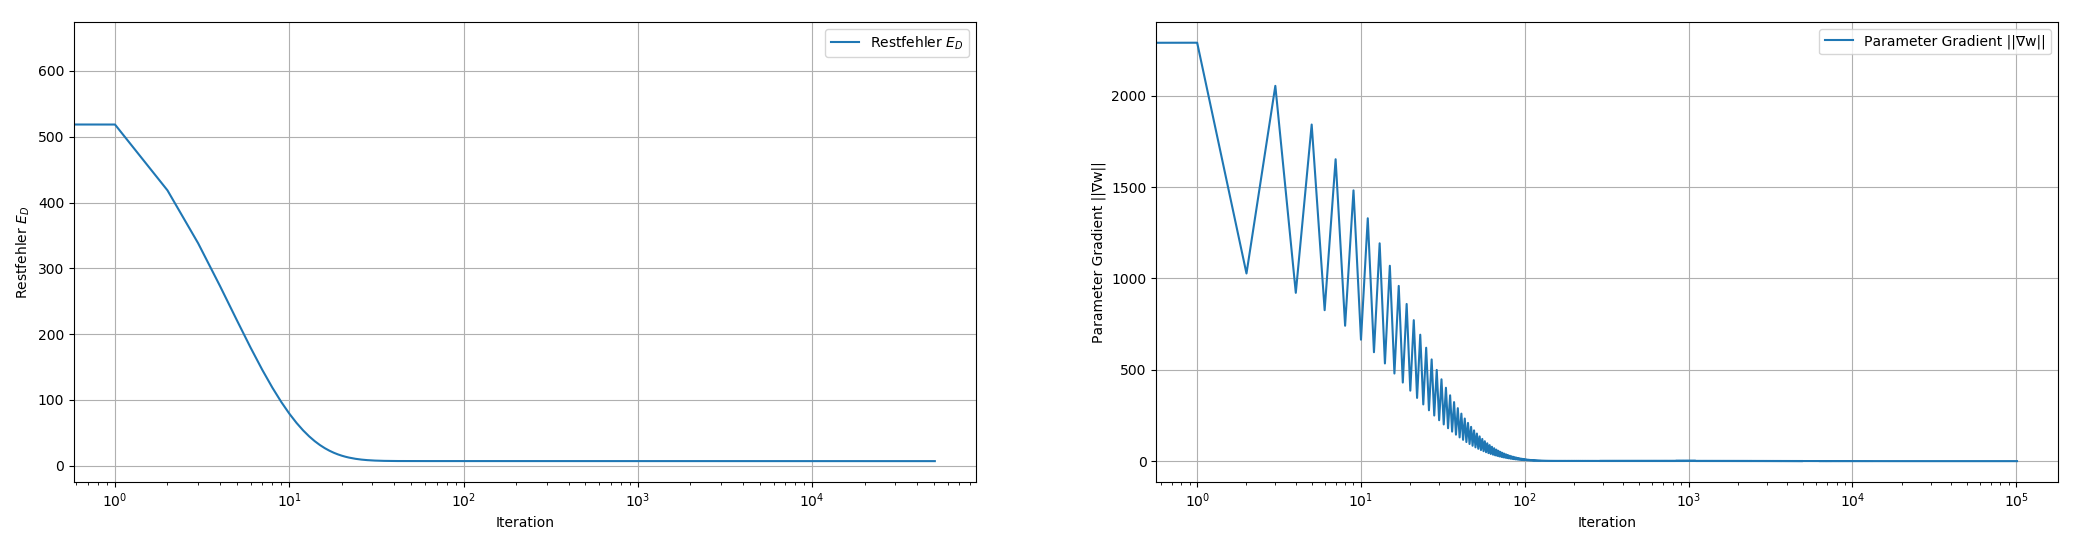
\includegraphics[width=\textwidth]{Momentum_0_0_Error_10e-12_Crop}
  \caption{Beispielfit mit $\gamma=0$}
\end{figure}
\begin{figure}[H]
  \centering
  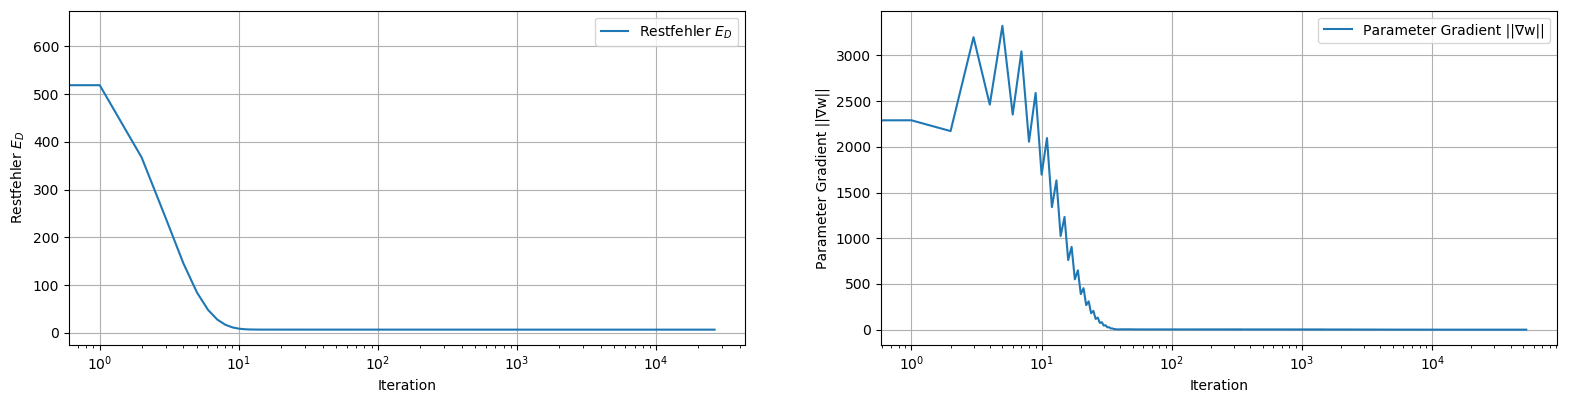
\includegraphics[width=\textwidth]{Momentum_0_5_Error_10e-12_Crop}
  \caption{Beispielfit mit $\gamma=0.5$}
\end{figure}
\begin{figure}[H]
  \centering
  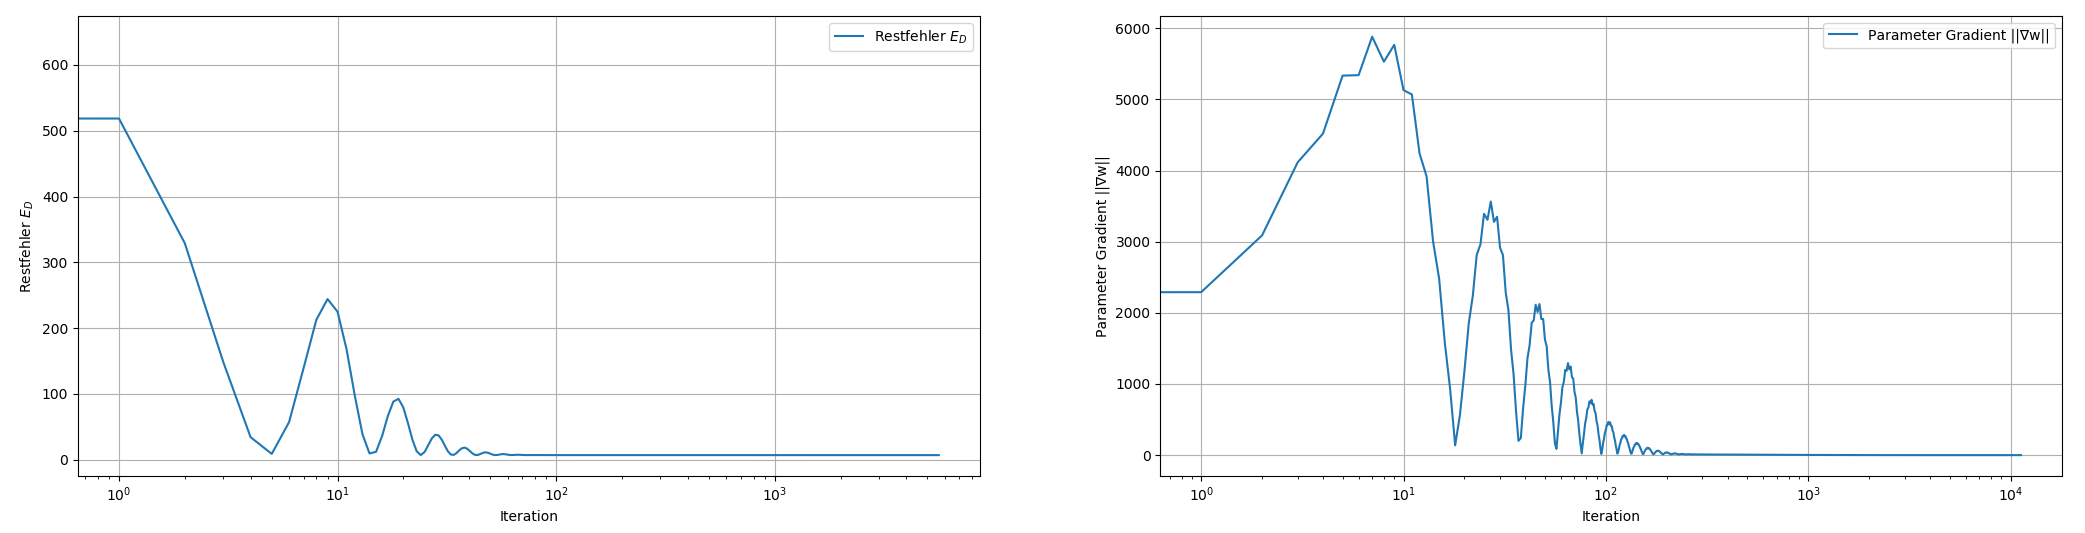
\includegraphics[width=\textwidth]{Momentum_0_9_Error_10e-12_Crop}
  \caption{Beispielfit mit $\gamma=0.9$}
\end{figure}

Es ist klar zu sehen, dass der oben genannte 'worst case' im Fall $\gamma=0.9$ eingetreten ist. Das vermeintlich bessere Konvergenzverhalten lag daran, dass ein sehr geringes $\varepsilon$ gewählt wurde. Erhöhen wir $\varepsilon$ auf beispielsweise \texttt{10e-3}, dann ergeben sich die folgenden Werte\footnote{Die GC Werte sind gestrichen, da sie sich nicht für alle Testdurchläufe bestimmen  ließen (\mintinline{Julia}|@time| liefert bei zu kurzen Durchläufen nicht zwingend alle Werte - evtl. liefert es keinen Wert falls während des Messvorgangs keine GC-Iteration vorlag. Die angegebenen Werte sind das Mittel aus drei Iterationen in denen ein GC-Wert vorlag.)}:

\begin{center}
  \begin{tabular}{cccccc}
    \toprule
    $\gamma$ & k bei Abbruch & Restfehler bei Abbruch  & Laufzeit & Gesamt allokierter & Garbage Collector\\
    &  nach k Iterationen & des Algorithmus & (in Sekunden) & Speicher (in MiB) & Zeitanteil (in \%) \\
    \midrule
        $0.0$ & $24$ & $10.216203809068343$ & $0.00581$ & $1.398$ & \sout{$61.54$} \\
        $0.5$ & $14$ & $6.813835951850837$  & $0.00570$ & $1.232$ & \sout{$48.19$} \\
        $0.9$ & $29$ & $36.63725946510655$  & $0.00680$ & $1.438$ & \sout{$60.92$} \\
  \end{tabular}
\end{center}

beziehungsweise folgende Graphen:

\begin{figure}[H]
  \centering
  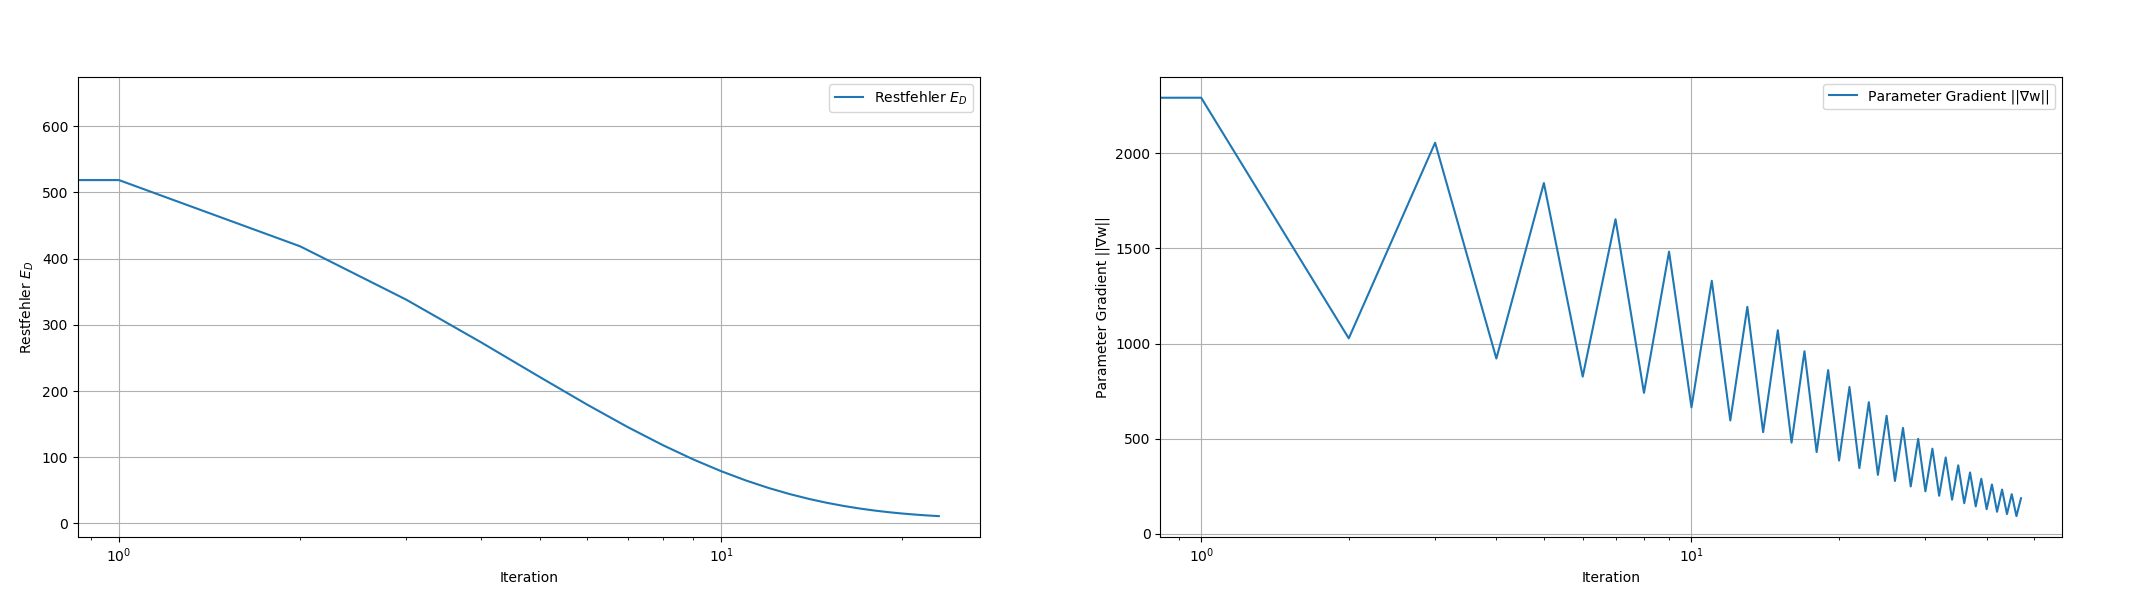
\includegraphics[width=\textwidth]{Momentum_0_0_Error_10e-3}
  \caption{Beispielfit mit $\gamma=0$}
\end{figure}
\begin{figure}[H]
  \centering
  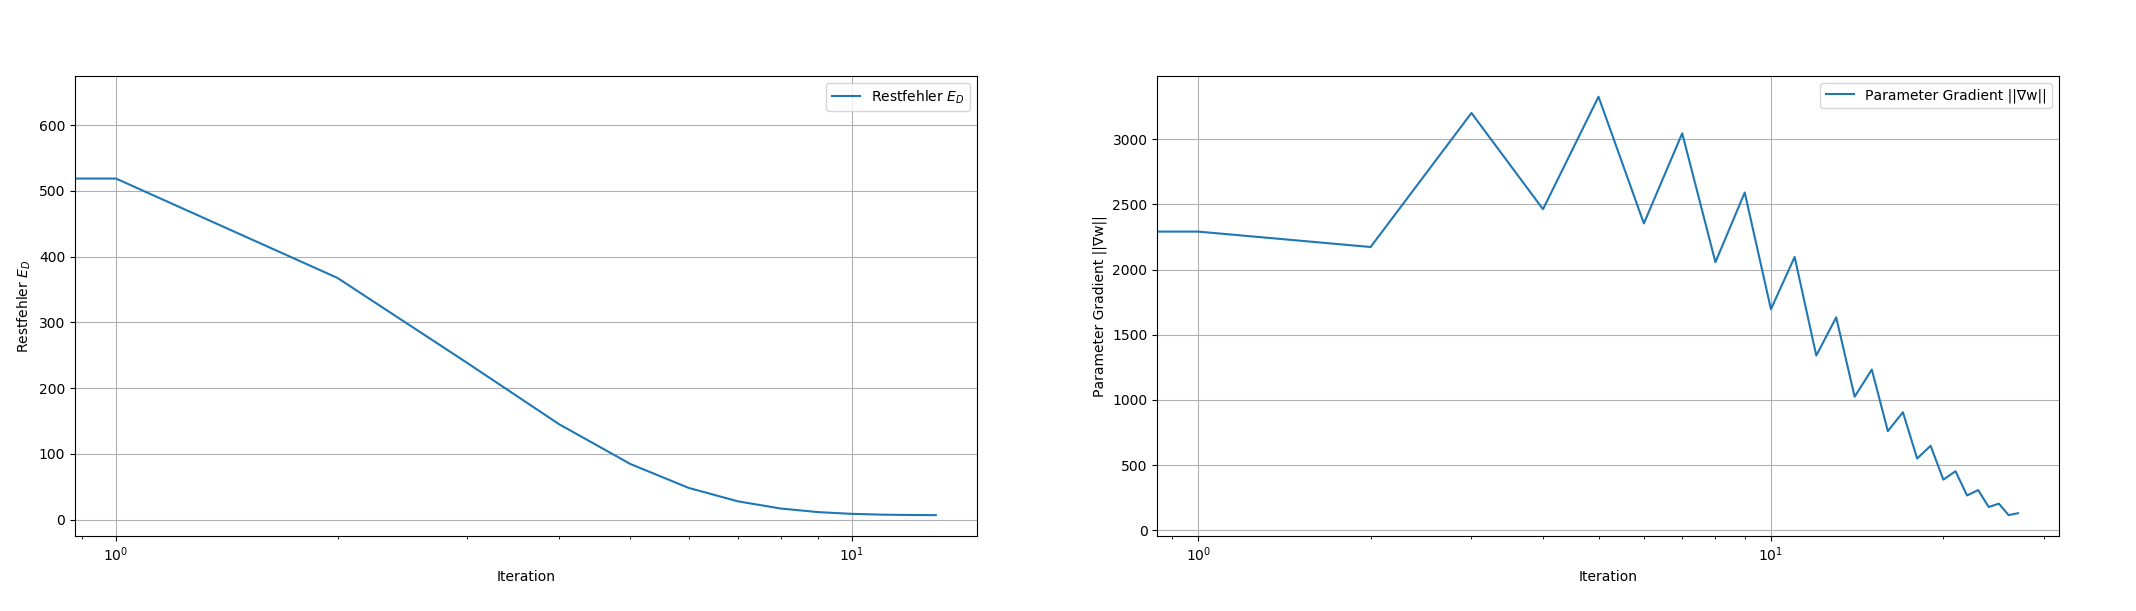
\includegraphics[width=\textwidth]{Momentum_0_5_Error_10e-3}
  \caption{Beispielfit mit $\gamma=0.5$}
\end{figure}
\begin{figure}[H]
  \centering
  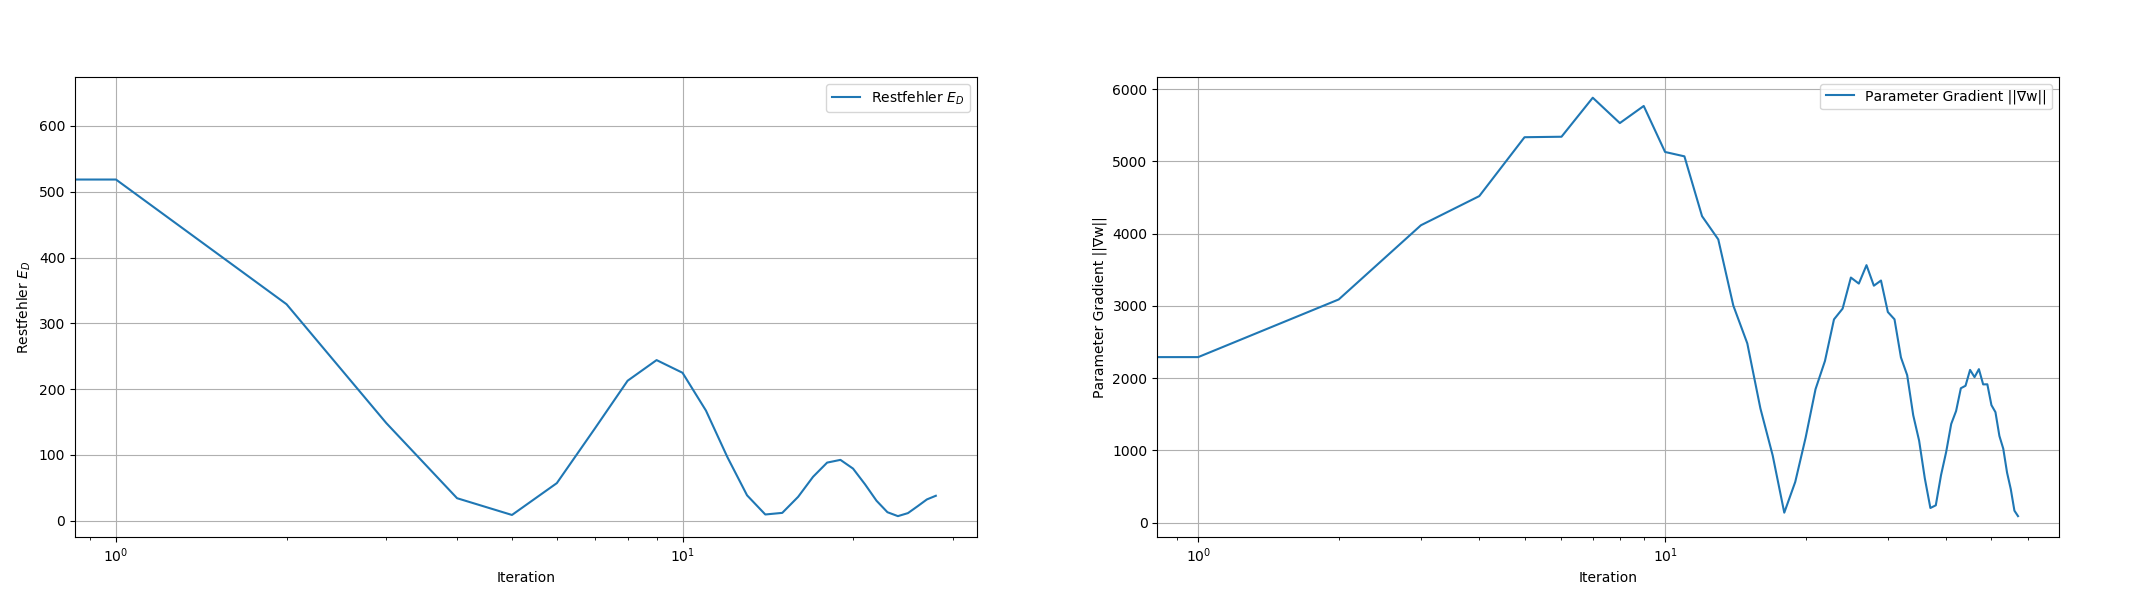
\includegraphics[width=\textwidth]{Momentum_0_9_Error_10e-3}
  \caption{Beispielfit mit $\gamma=0.9$}
\end{figure}

Das Momentumverfahren wirkt sich hier also teils positiv und teils negativ aus - bei der Wahl der Parameter ist vorsicht geboten.

\subsection{Tichonow Regularisierung}
Eine weitere Möglichkeit der Verbesserung des Verfahrens ist die \emph{Tichonow Regularisierung}. Das Ziel dieses Verfahrens ist es, die Stabilität des Modells zu verbessern. Dabei wird das Minimierungsproblem wie folgt neu formuliert:
$$
  \min_{\mathbf{w} \in \mathbb{R}^M} \frac{1}{2}\sum_{n=1}^{N}(\mathbf{t}_n - y(\mathbf{w}, X_n))^2 + \omega ||\mathbf{w}||^2_2.
$$
Es werden also zu große Werte in $\mathbf{w}$ ''bestraft''. Hierbei ist $\omega$ ein neuer Hyperparameter welcher festlegt wie ''wichtig'' die Minimierung des Parametervektors ist. Die neue partielle Ableitung ist damit:
$$
  \frac{\partial E_{D, decay}}{\partial \mathbf{w}_k} = - \sum_{n=1}^N \Phi(k, X_n) \cdot (\mathbf{t}_n - y(\mathbf{w}, \Phi, X_n)) - \omega \mathbf{w}_k
$$

Die erforderlichen Änderungen am Code sind das Durchschleifen des Parameters $\omega$ und die Anpassung der partielle Ableitung:

\begin{listing}[H]
  \begin{minted}[bgcolor=bg]{Julia}
    """Derivative of E_D with respect to 𝐰ₖ
    # Args:
        Φ(k, 𝐱ₙ): Basis function
        𝐗: Set of inputs 𝐱ₙ where 𝐱ₙ is an input vector to Φ
        t: corresponding target values for each 𝐱ₙ
        𝐰: Parameters
        k: Index for 𝐰ₖ in respect to which the derivative is taken
        ω: Weight decay factor
    """
    function ∂E_D∂w_k(Φ::Function,
      𝐗::Matrix{<:Number},
      t::Vector{<:Number},
      𝐰::Vector{<:Number},
      k::Integer,
      ω::Real)::Number
        N = size(t)[1]
        - Σ(1, N, n->Φ(k, 𝐗[n, :]) * (t[n] - y(𝐰, Φ, 𝐗[n,:])) - ω*𝐰[k])
    end
  \end{minted}
  \caption{Funktion \mintinline{julia}|∂E_D∂w_k| mit Tichonow Regularisierung}
  \label{listing:decay}
\end{listing}

\subsection{Ausblick auf den Broyden–Fletcher–Goldfarb–Shanno Algorithmus}

Der Broyden–Fletcher–Goldfarb–Shanno - oder kurz BFGS - Algorithmus, ist ein Optimierungsverfahren aus der Gruppe der Quasi-Newton Verfahren. Nach \cite{Dai} ist BFGS der effizienteste Vertreter dieser Gruppe; so findet sich das Verfahren auch in vielen professionellen Softwaretoolboxes und Programmiersprachen wie z.B. R, Matlab oder auch SciPy wieder.
Ziel ist das lösen des Optimierungsproblems $\min_{\mathbf{x} \in \mathbb{R}^n} f(\mathbf{x})$ mit $f: \mathbb{R}^n \rightarrow \mathbb{R}$.
Beginnend mit einem Startwert $\mathbf{x}_0$ und einer Näherung der Hesse Matrix $B_0 := I_n$ werden folgende Schritte abgearbeitet. Dabei konvergiert $\mathbf{x}_k$ gegen die Lösung des Problems.

\begin{enumerate}
  \item{ Bestimmen einer Abstiegsrichtung $\mathbf{p}_k$ durch lösen des LGS $B_k \cdot \mathbf{p}_k = - \nabla f(\mathbf{x}_k)$. }
  \item{ Sei $g_k: \mathbb{R} \rightarrow \mathbb{R}$ definiert durch $\alpha \mapsto f(x_k + \alpha \cdot p_k)$, dann ist die Schrittweite $\alpha_k > 0$ gegeben durch $\alpha_k = \arg \min_{\alpha \in \mathbb{R}} \frac{\partial g_k}{\partial \alpha}$.\\Dieses Minimierungsproblem wird mittels eines Liniensuchverfahrens (in der Implementierung wird hier zwecks Einfachheit das Gradientenabstiegsverfahren gewählt - andere mögliche Kandidaten wären z.B. Newton Verfahren oder das CG-Verfahren) gelöst - wobei nur ein lokales Minimum gesucht wird\cite{Dai}.}
  \item {Setzen von $\mathbf{s}_k = \alpha_k \cdot \mathbf{p}_k$ und $\mathbf{x}_{k+1} = \mathbf{x}_k + \mathbf{s}_k$.}
  \item {Berechnung von $\mathbf{y}_k = \nabla f(\mathbf{x}_{k+1}) - \nabla f(\mathbf{x}_k)$.}
  \item {Neue Näherung der Hesse Matrix $B$ nach der Rekursionsvorschrift $B_{k+1} = B_k + \frac{\mathbf{y}_k \mathbf{y}_k^T}{\mathbf{y}_k^T \mathbf{s}_k} - \frac{B_k \mathbf{s}_k \mathbf{s}_k^T B_k}{\mathbf{s}_k^T B_k \mathbf{s}_k}$ bestimmen.}
\end{enumerate}

Schritt 2 lässt sich so visualisieren, dass man die durch die Funktion beschriebene Figur mit der von Gradient und y-Achse aufgespannten Ebene schneidet - und dann das der aktuellen Position näheste lokale Minimum der dabei entstehenden Kurve sucht. Aus dieser Überlegung folgt direkt, dass für einfache Probleme(z.B. $f(x,y) = x^2 + y^2$)(bei korrekter Parameterwahl) nach nur einem Schritt bereits eine Lösung gefunden wird.

\begin{figure}[t]
  \centering
  \includegraphics[width=.5\textwidth]{octave_contour_mod}
  \caption{Contourplot mit Visualisierung zu Schritt 2. Der rote Punkt zeigt die Startposition $x_k$, die blaue Linie einen Teil der durch $x_k + \alpha p_k$ beschriebenen Geraden. Durch eine eindimensionale Optimierung wird dann $\alpha_k$ so gewählt, dass man bei einem Minimum(orange/braune Ellipse) landet. Originalbild von \url{https://octave.sourceforge.io/octave/function/images/contour_101.png}.}
\end{figure}

In Schritt 2 wird die Ableitung von $f(x_k + \alpha p_k)$ nach $\alpha$ benötigt - um diese nicht immer bestimmen zu müssen, werden wir sie einfach numerisch nähern. Die Funktion \mintinline{Julia}|numeric_differentiation(f, h) = x -> (f(x + h) - f(x - h)) / (2 * h)| bestimmt mittels des zentralen Differenzquotienten die Ableitung einer eindimensionalen Funktion $f$.

Zum line search wählen wir zu Demozwecken den bereits bekannten Gradientenabstieg - diesmal jedoch in allgemeiner Ausführung und ohne Regularisierung etc..

\begin{listing}[H]
  \begin{minted}[bgcolor=bg]{Julia}
    """Optimize some function f
    # Args:
        ∇f: Gradient of f
        x_0: Initial guess
        η: learning rate
        ε: cancellation tolerance
        max_iters: maximum number of iterations
    """
    function gradient_descent(∇f::Function,
      x_0,
      η::Number,
      ε::Number,
      max_iters::Integer)
        x_k = x_0
        count = 0
        for _ = 1:max_iters
            if any(isnan.(x_k))
                error("Encoutered NaN")
            end
            if any(isinf.(x_k))
                error("Encoutered Inf")
            end
            count += 1
            p_k = -∇f(x_k)
            if norm(∇f(p_k)) < ε
                break
            end
            x_k += η * p_k
        end
        x_k
    end
  \end{minted}
  \caption{Funktion \mintinline{julia}|gradient_descent|}
  \label{listing:decay}
\end{listing}


Die liniensuchfunktionsagnostische Implementierung des BFGS-Algorithmus ist dann wie folgt:

\begin{listing}[H]
  \begin{minted}[bgcolor=bg]{Julia}
    """BFGS Optimization Algorithm

    # Args:
        ∇f: Gradient of function to optimize
        x_0: Initial guess for optimal value
        iters: Maximum number of iterations before cancellation
        line_search: Line search function that's used
        ε: Optimization stops once the norm of the gradient is below this value
    """
    function BFGS(
      f::Function,
      ∇f::Function, 
      x_0::Vector{<:Number}, 
      iters::Integer,
      line_search::Function,
      ε = 10e-12::Real)
        n = size(x_0)[1]
        x_k = x_0
        B_k = Matrix{typeof(x_0[1])}(I, n, n)

        for i = 1:iters
            if norm(∇f(x_k)) < ε
                break
            end
            # Step 1: obtain direction p_k by solving
            # B_k ∙ p_k = - (gradient of f at x_k)
            p_k = B_k \ -∇f(x_k)
            # Step 2.: Find stepsize α_k such that
            # α_k = arg min ∂f(x_k + α_k * p_k)/∂α
            α_k = line_search(numeric_differentiation(α->(f(x_k + α * p_k)), 10e-10))
            # Step 3.
            s_k = α_k * p_k
            x_k_prime = x_k + s_k
            # Step 4.
            y_k = ∇f(x_k_prime) - ∇f(x_k)
            # Step 5.
            B_k += (y_k * y_k') / (y_k' * s_k) +
              - (B_k * s_k * s_k' * B_k) / (s_k' * B_k * s_k)
            x_k = x_k_prime
        end
        x_k
    end
  \end{minted}
  \caption{Funktion \mintinline{julia}|BFGS|}
  \label{listing:decay}
\end{listing}

Betrachten wir nun beispielsweise die Funktion $f(x) = \frac{x^5}{5000} + \frac{21 x^4}{4000} + \frac{17 x^3}{375} + \frac{293 x^2}{1000} + \frac{521 x}{1000}$ mit $\nabla f(x) = \frac{x^4}{1000} + \frac{21x^3}{1000} + \frac{17 x^2}{125} + \frac{293 x}{500} + \frac{521}{1000}$ und führen mit ihr BFGS aus
\mintinline{Julia}|BFGS(f, ∇f, [0], 500, ∇f -> gradient_descent(∇f, 10e-10, 1, 1e-10, 1000), 10e-5)|,
erhalten wir nach zwei Iterationen ein lokales Minimum bei $x=-1.1408$.

Eine recht simple Optimierung der Implementierung ist in Schritt 1 möglich. Hier wird aktuell der \mintinline{Julia}|\|-Operator\footnote{\url{https://docs.julialang.org/en/v1/stdlib/LinearAlgebra/}} eingesetzt. Dies ist zwar eine valide Lösung, jedoch nicht besonders effizient. Stattdessen kann hier nach \cite{wiki:BFGS} die Sherman–Morrison–Woodbury Formel angewandt werden um die Inverse rekursiv zu beschreiben. Die Rekursionsvorschrift lautet:
$$
B_{k+1}^{-1} = B_k^{-1} + \frac{(\mathbf{s}_k^T \mathbf{y}_k + \mathbf{y}_k^T B_k^{-1} \mathbf{y}_k)(\mathbf{s}_k \mathbf{s}_k^T)}{(\mathbf{s}_k^T \mathbf{y}_k)^2} - \frac{B_k^{-1} \mathbf{y}_k \mathbf{s}_k^T + \mathbf{s}_k \mathbf{y}_k^T B_k^{-1}}{\mathbf{s}_k^T \mathbf{y}_k}.
$$
Für die erste Iteration gilt $B_1 = I_n$, und daher auch $p_1 = -\nabla f(\mathbf{x}_k)$ bzw. $B_1^{-1} = I_n$.

Mit dem fertigen BFGS kann man nun \mintinline{Julia}|fit_linear_model| dahingehend erweitern/ändern, dass es intern BFGS nutzt. Außerdem öffnet BFGS die Tür zu anderen Verfahren wie z.B. logistischer Regression.

\newpage

\appendix

\section{Performancemessung}\label{appendix:measure}

Das Laufzeitverhalten wurde mittels des built-in Macros \mintinline{julia}|@time| gemessen. Testsystem war ein Intel i7-4790k@3.8GHz unter Linux Mint 19. Auswertung der Ausgabe des Macros erfolgte mittels des Python Scripts in Listing \ref{listing:measure}. Die Tabellenwerte ergeben sich als arithmetisches Mittel von 100 Aufrufen der Funktion \mintinline{julia}|fit_linear_model|.

\begin{listing}[H]
  \begin{minted}[bgcolor=bg, linenos]{Python}
    from statistics import mean
    import re
    
    """Regex to capture different components
    Examples:
      0.000103 seconds (818 allocations: 87.328 KiB)
      0.000388 seconds (3.78 k allocations: 412.406 KiB)
      0.598357 seconds (2.02 M allocations: 102.555 MiB, 3.13% gc time)
    """
    RE = r"\s*(?P<time>\d+\.\d*) seconds \((?:(?P<allocs>\d+(?:\.\d*)?)"\
        r"(?: (?P<allocsuffix>M|k))?) allocations: (?:(?P<mem>\d+\.\d*)"\
        r"(?: (?P<memsuffix>(?:KiB|MiB)))?)(?:, (?P<gctime>\d+\.\d*)% gc time)?\)"
    
    MEMORY_FACTOR = {None: 1, "MiB": 1, "KiB": 1 / 1024}
    

    def get_and_parse():
        try:
            while line := input():
                match = re.match(RE, line)
                time = float(match["time"])
                mem = float(match["mem"]) * MEMORY_FACTOR[match["memsuffix"]]
                if (gc_time:=match["gctime"]) is not None:
                    gc = float(gc_time)
                else:
                    gc = None
                yield (time, mem, gc)
        except EOFError: return None
    

    time, memory, gc_time = zip(*(x for x in get_and_parse()))
    gc_time = list(filter(lambda x: x is not None, gc_time))
    print(
        f"Time: {mean(time):.5f} s, RAM: {mean(memory):.3f} MiB, "\
        f"GC-time: {mean(gc_time):.2f} % (got {len(gc_time)} gc values)")

  \end{minted}
  \caption{Python Script zur \mintinline{julia}|@time| Auswertung}
  \label{listing:measure}
\end{listing}
Das Script wurde für Python 3.8.0 geschrieben und ist auch nicht in älteren Versionen lauffähig(hierzu müsste man die Assignment Expressions ersetzen). Der Code gestaltet sich etwas komplizierter, da \mintinline{Julia}|@time| je nach Anzahl der Allokationen ein verschiedenes Ausgabeformat wählt. Daher seien spezielle Sprachfeatures und nicht-triviale Codepassagen hier kurz erläutert:

Hintereinanderstehende Strings werden in Python automatisch verkettet - \texttt{\textbackslash} erlaubt es lange Zeilen umzubrechen. Der \mintinline{Python}|:=| Operator führt eine \emph{Assignment Expression}\footnote{\url{https://www.python.org/dev/peps/pep-0572/}} aus. Diese funktionieren ähnlich einer Zuweisung in C oder auch ALGOL 68; in Kombination mit \mintinline{Python}|while| ergibt sich ein Konstrukt ähnlich einem \mintinline{Rust}|while let Some(x) = ...| in Rust. Die Funktion \mintinline{Python}|get_and_parse| fungiert als Generator\footnote{\url{https://docs.python.org/3/howto/functional.html}} welcher über stdin die Messwerte einliest, parset und als Dreiertupel zurückgibt. Für eine zweidimensionale Collection \texttt{c} in row-major order wandelt \mintinline{Python}|zip(*c)| diese in eine in column-major order um. Bei \texttt{RE} handelt es sich um eine Regular Expression\footnote{\url{https://docs.python.org/3/library/re.html}} welche in diesem Fall alle Eingabeformate unterscheiden und die einzelnen Komponenten automatisch extrahieren kann. Bei \mintinline{Python}|(x for x in get_and_parse())| in Zeile \texttt{31} handelt es sich um eine \emph{Generator Expression}\footnote{\url{https://www.python.org/dev/peps/pep-0289/}} welche ähnlich zu einer List Comprehension in Python, Haskell, Erlang oder auch Julia funktioniert - jedoch im Effekt eine Art Lazy Evaluation realisiert. Diese Generator Expression wird hier nur benötigt um das Entpacken mittels \texttt{*} zu ermöglichen. Die Konvertierung des Generators zu einer Liste in Zeile 32 ist leider nötig (sofern man keine eigene Funktion schreibt, welche gleichzeitig die Länge bestimmt und das Mittel berechnet) da der Generator beim Aufruf von \mintinline{Python}|len| oder \mintinline{Python}|mean| sonst verbraucht würde.
Die Nutzung erfolgt dann beispielsweise mit \mintinline{Bash}{$ julia Tests.jl | python3.8 measure.py}.

\bibliographystyle{alphadin}
\bibliography{Quellen}

\end{document}